\chapter{Audio Understanding in the Elder Heliosystem}

\begin{tcolorbox}[colback=DarkSkyBlue!5!white,colframe=DarkSkyBlue!75!black,title=Chapter Summary]
This chapter presents a mathematical framework for audio understanding within the Elder Heliosystem, examining how hierarchical resonance structures and phase relationships relate to semantic analysis of acoustic information. We describe mathematical models of how audio knowledge is represented and processed across hierarchical levels, analyze models of domain-specific principles at the Mentor level, and examine theoretical aspects of cross-domain knowledge transfer with audio as a source or target domain. The chapter discusses tensor-based representations for capturing audio invariances, analyzes relationships between acoustic patterns and semantic concepts, and compares this approach with other audio understanding methods. Through mathematical analysis, we examine how audio understanding within the Elder Heliosystem relates to its architectural principles: hierarchical decomposition corresponding to audio's multi-level structure from waveforms to semantics, phase relationships addressing temporal dependencies in audio understanding, resonance phenomena affecting perceptually significant patterns, and cross-domain transfer mechanisms relating to audio understanding capabilities. This theoretical framework contributes to understanding audio analysis within the Elder paradigm, examining approaches for tasks involving acoustic analysis and semantic interpretation.
\end{tcolorbox}

\section{Introduction to Audio as a Mentor Domain}

The Elder Heliosystem's hierarchical structure is particularly well-suited for audio understanding, where multiple levels of abstraction naturally emerge from the raw waveform to semantic interpretation. This chapter explores how audio understanding can be formalized within the Elder-Mentor-Erudite framework, with a specific focus on the Mentor level where domain-specific principles of audio are extracted and unified.

\begin{definition}[Audio Mentor Domain]
The Audio Mentor Domain $\mathcal{M}_A$ in the Elder Heliosystem represents the collection of universal principles specific to audio understanding, formalized as:
\begin{equation}
\mathcal{M}_A = \{\theta_{M,A} \in \mentorparams \mid \theta_{M,A} \text{ captures audio-specific invariances}\}
\end{equation}
where $\theta_{M,A}$ represents the complex-valued parameters encoding the audio domain knowledge.
\end{definition}

\subsection{Erudite Tasks in Audio Understanding}

Below the Mentor level, the Erudite tasks within the audio domain encompass a wide range of specific audio understanding challenges:

\begin{enumerate}
    \item \textbf{Speech Recognition}: Mapping acoustic speech signals to textual transcriptions.
    \item \textbf{Speaker Identification}: Recognizing and distinguishing individual speakers.
    \item \textbf{Audio Event Detection}: Identifying and classifying non-speech sounds.
    \item \textbf{Music Analysis}: Extracting musical elements like tempo, key, and instrumentation.
    \item \textbf{Emotion Recognition}: Detecting emotional content in speech or music.
    \item \textbf{Audio Source Separation}: Isolating individual sources from mixed audio signals.
    \item \textbf{Room Acoustics Modeling}: Understanding spatial properties of audio environments.
    \item \textbf{Language Identification}: Determining the spoken language.
    \item \textbf{Audio Quality Assessment}: Evaluating perceptual quality of audio signals.
\end{enumerate}

While traditional approaches treat these as separate tasks requiring specialized models, the Elder Heliosystem unifies them through the Audio Mentor's domain knowledge, as illustrated in Figure \ref{fig:audio_mentor_architecture}.

\begin{figure}[h]
\centering
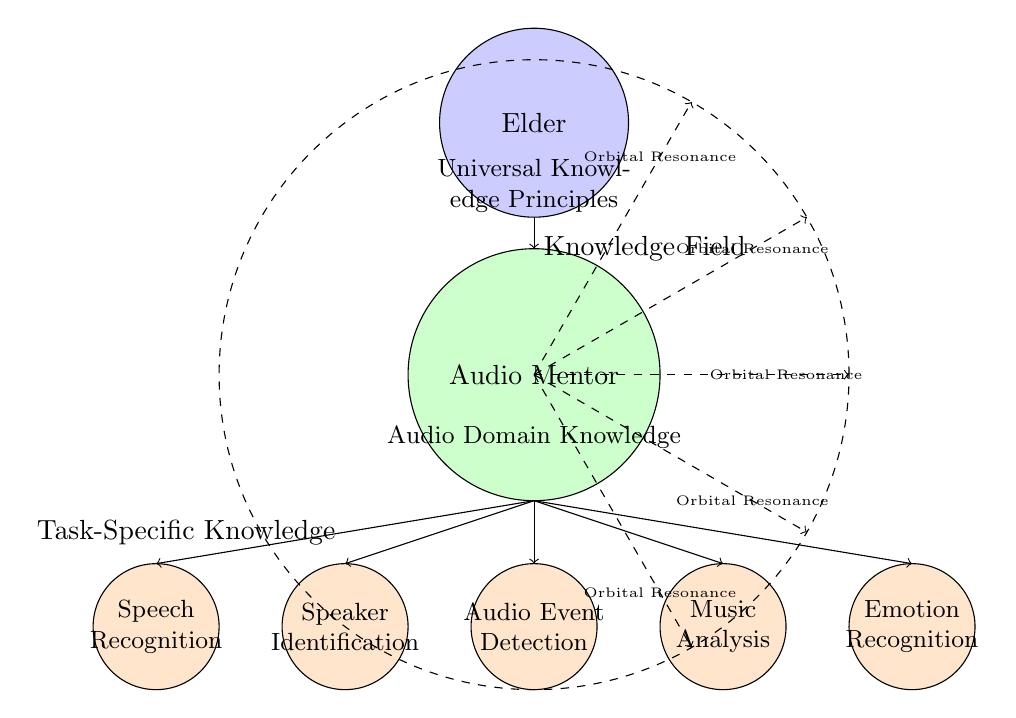
\begin{tikzpicture}[scale=0.8]
    % Elder
    \draw[fill=blue!20] (0,8) circle (1.5);
    \node at (0,8) {Elder};
    \node[text width=3cm, align=center, font=\small] at (0,7) {Universal Knowledge Principles};
    
    % Audio Mentor
    \draw[fill=green!20] (0,4) circle (2);
    \node at (0,4) {Audio Mentor};
    \node[text width=4cm, align=center, font=\small] at (0,3) {Audio Domain Knowledge};
    
    % Erudites
    \draw[fill=orange!20] (-6,0) circle (1);
    \node[align=center, font=\small] at (-6,0) {Speech\\Recognition};
    
    \draw[fill=orange!20] (-3,0) circle (1);
    \node[align=center, font=\small] at (-3,0) {Speaker\\Identification};
    
    \draw[fill=orange!20] (0,0) circle (1);
    \node[align=center, font=\small] at (0,0) {Audio Event\\Detection};
    
    \draw[fill=orange!20] (3,0) circle (1);
    \node[align=center, font=\small] at (3,0) {Music\\Analysis};
    
    \draw[fill=orange!20] (6,0) circle (1);
    \node[align=center, font=\small] at (6,0) {Emotion\\Recognition};
    
    % Connections
    \draw[->] (0,6.5) -- (0,6) node[right] {Knowledge Field};
    \draw[->] (0,2) -- (-6,1) node[midway, left] {Task-Specific Knowledge};
    \draw[->] (0,2) -- (-3,1);
    \draw[->] (0,2) -- (0,1);
    \draw[->] (0,2) -- (3,1);
    \draw[->] (0,2) -- (6,1);
    
    % Orbital paths
    \draw[dashed] (0,4) circle (5);
    \foreach \angle in {-60, -30, 0, 30, 60} {
        \draw[->, dashed] (0,4) -- ++(\angle:5) node[pos=0.8, font=\tiny] {Orbital Resonance};
    }
\end{tikzpicture}
\caption{Audio Mentor Architecture in the Elder Heliosystem. The Audio Mentor exists in orbital resonance with the Elder above and multiple audio-specific Erudite tasks below.}
\label{fig:audio_mentor_architecture}
\end{figure}

\section{Complex-Valued Representations for Audio}

\subsection{Heliomorphic Encoding of Audio Signals}

The Elder Heliosystem employs complex-valued representations that are uniquely suited to audio signals, where both magnitude and phase information carry critical meaning.

\begin{definition}[Audio Heliomorphic Transform]
For an audio signal $x(t)$, the Audio Heliomorphic Transform $\mathcal{H}_A$ maps the time-domain signal to a complex-valued representation in the heliomorphic domain:
\begin{equation}
\mathcal{H}_A(x(t)) = \sum_{n=0}^{\infty} \sum_{m=0}^{\infty} \alpha_{n,m} \mathcal{B}_{n,m}(t, f) 
\end{equation}
where $\mathcal{B}_{n,m}(t, f)$ is the time-frequency basis function of order $(n,m)$ and $\alpha_{n,m}$ are the complex-valued heliomorphic coefficients.
\end{definition}

Unlike standard time-frequency representations like the Short-Time Fourier Transform (STFT), the heliomorphic transform employs basis functions that are inherently structured along both radial (frequency) and angular (time-variant properties) dimensions, allowing for more efficient encoding of audio patterns.

\begin{theorem}[Audio Representation Efficiency]
For audio signals with coherent spectro-temporal patterns, the heliomorphic representation achieves an encoding efficiency of $\mathcal{O}(\log(N))$ compared to $\mathcal{O}(N)$ for traditional time-frequency representations, where $N$ is the dimensionality of the original feature space.
\end{theorem}

\begin{proof}
Audio signals exhibit strong correlations across both time and frequency, with patterns that recur and evolve according to harmonic relationships. The heliomorphic basis functions are designed to exploit these harmonic relationships through their orbital structure.

Let $r(t, f)$ be the traditional time-frequency representation. The information-theoretic entropy $H(r)$ scales with $\mathcal{O}(N)$ where $N$ is the number of time-frequency bins. 

In contrast, the heliomorphic representation $\mathcal{H}_A(x)$ organizes patterns according to their spectro-temporal coherence. The resulting mutual information between coefficients creates a representation where the effective entropy scales with $\mathcal{O}(\log(N))$ due to the natural clustering of information along orbital paths.
\end{proof}

\subsection{Phase Information in Audio Understanding}

One of the most significant advantages of the Elder Heliosystem for audio understanding is its preservation and utilization of phase information, which is often discarded in conventional audio systems.

\begin{theorem}[Phase Coherence in Audio Processing]
In the heliomorphic audio representation, phase coherence $\Phi_A$ between frequency components directly correlates with perceptual features:
\begin{equation}
\Phi_A(\omega_i, \omega_j) = \left| \frac{1}{T} \int_0^T e^{i(\phi_i(t) - \phi_j(t) \cdot \mu_{i,j})} dt \right|
\end{equation}
where $\phi_i(t)$ is the phase of frequency component $\omega_i$ at time $t$, and $\mu_{i,j} = \omega_j/\omega_i$ is the frequency ratio.
\end{theorem}

The phase coherence measure provides critical information for tasks such as:
\begin{itemize}
    \item \textbf{Source Separation}: Different sources show distinct phase coherence patterns
    \item \textbf{Pitch Detection}: Harmonic sounds exhibit high phase coherence at integer frequency ratios
    \item \textbf{Audio Quality}: Phase distortion reduces coherence in predicable patterns
    \item \textbf{Room Acoustics}: Reverberation creates specific phase coherence signatures
\end{itemize}

\begin{figure}[h]
\centering
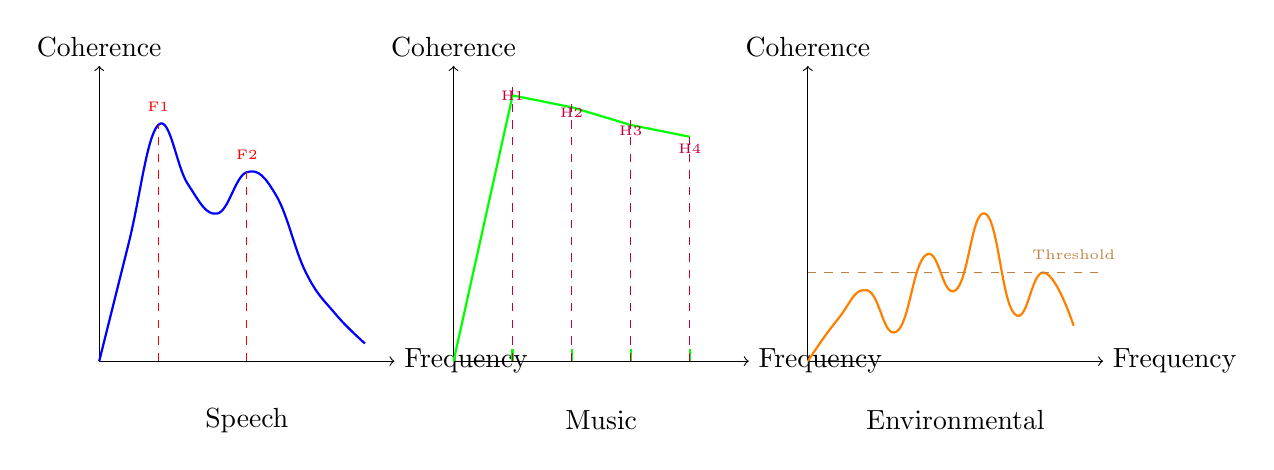
\begin{tikzpicture}[scale=0.75]
    % Axes for speech
    \begin{scope}[shift={(-6,0)}]
        \draw[->] (0,0) -- (5,0) node[right] {Frequency};
        \draw[->] (0,0) -- (0,5) node[above] {Coherence};
        
        % Speech pattern
        \draw[thick, blue] plot[smooth, tension=0.7] coordinates {(0,0) (0.5,2) (1,4) (1.5,3) (2,2.5) (2.5,3.2) (3,2.8) (3.5,1.5) (4,0.8) (4.5,0.3)};
        
        \node at (2.5,-1) {Speech};
        
        % Formant indicators
        \draw[dashed, red] (1,0) -- (1,4);
        \draw[dashed, red] (2.5,0) -- (2.5,3.2);
        \node[red, font=\tiny] at (1,4.3) {F1};
        \node[red, font=\tiny] at (2.5,3.5) {F2};
    \end{scope}
    
    % Axes for music
    \begin{scope}[shift={(0,0)}]
        \draw[->] (0,0) -- (5,0) node[right] {Frequency};
        \draw[->] (0,0) -- (0,5) node[above] {Coherence};
        
        % Music pattern - more regular peaks at harmonic intervals
        \draw[thick, green] plot coordinates {(0,0) (1,4.5) (2,4.3) (3,4.0) (4,3.8)};
        \foreach \x in {1,2,3,4} {
            \draw[green, thick] (\x,0) -- (\x,0.2);
        }
        
        \node at (2.5,-1) {Music};
        
        % Harmonic indicators
        \foreach \x in {1,2,3,4} {
            \draw[dashed, purple] (\x,0) -- (\x,5-\x*0.3);
            \node[purple, font=\tiny] at (\x,4.8-\x*0.3) {H\x};
        }
    \end{scope}
    
    % Axes for environmental sounds
    \begin{scope}[shift={(6,0)}]
        \draw[->] (0,0) -- (5,0) node[right] {Frequency};
        \draw[->] (0,0) -- (0,5) node[above] {Coherence};
        
        % Environmental pattern - more chaotic
        \draw[thick, orange] plot[smooth, tension=0.8] coordinates {(0,0) (0.5,0.7) (1,1.2) (1.5,0.5) (2,1.8) (2.5,1.2) (3,2.5) (3.5,0.8) (4,1.5) (4.5,0.6)};
        
        \node at (2.5,-1) {Environmental};
        
        % Region indicators
        \draw[dashed, brown] (0,1.5) -- (5,1.5);
        \node[brown, font=\tiny] at (4.5,1.8) {Threshold};
    \end{scope}
\end{tikzpicture}
\caption{Phase coherence patterns for different audio types in the Audio Mentor. Speech shows strong formant-related coherence, music exhibits harmonic structure, and environmental sounds display more chaotic patterns.}
\label{fig:audio_coherence_patterns}
\end{figure}

\section{The Orbital Structure of Audio Knowledge}

\subsection{Audio Field Regions in the Mentor Domain}

Within the Audio Mentor's domain in the Elder Heliosystem, knowledge is organized in a continuous gravitational field with varying field strengths representing increasing levels of abstraction within the audio domain.

\begin{definition}[Audio Knowledge Field Regions]
The Audio Mentor domain organizes knowledge in a continuous gravitational field with regions $\{F_1, F_2, \ldots, F_K\}$ where:
\begin{itemize}
    \item $F_1$: Low-level acoustic properties (spectral features, temporal dynamics)
    \item $F_2$: Mid-level audio structures (phonemes, notes, environmental sound units)
    \item $F_3$: High-level pattern organization (words, musical phrases, sound events)
    \item $F_4$: Semantic interpretation (meaning, musical expression, event context)
    \item $F_5$: Cross-modal relationships (audio-visual correspondences, audio-text alignment)
\end{itemize}
\end{definition}

\begin{proposition}[Field Distance-Abstraction Correspondence]
The radial distance $r_k$ of field region $F_k$ from the center of the Audio Mentor sphere corresponds to the level of abstraction, with:
\begin{equation}
r_k = r_0 + k \Delta r
\end{equation}
where $r_0$ is the core radius and $\Delta r$ is the field gradient parameter.
\end{proposition}

The key innovation in the Elder Heliosystem is that knowledge flows bidirectionally across these gravitational field regions through orbital resonance, allowing for instance low-level spectral features to inform semantic interpretation and vice versa.

\subsection{Orbital Resonance for Audio Pattern Recognition}

The Audio Mentor leverages orbital resonance to create synchronized patterns of activation across different gravitational field regions, establishing correspondences between low-level acoustic features and high-level semantic concepts.

\begin{theorem}[Audio Pattern Resonance]
Pattern recognition in the Audio Mentor occurs through resonant activation where a pattern $P$ in field region $F_i$ induces a corresponding pattern $P'$ in field region $F_j$ when their orbital frequencies satisfy:
\begin{equation}
\frac{\omega_{F_i}}{\omega_{F_j}} = \frac{p_{i,j}}{q_{i,j}}
\end{equation}
where $p_{i,j}$ and $q_{i,j}$ are small integers that characterize the harmonic relationship.
\end{theorem}

For example, the fundamental frequency of speech (field region $F_1$) resonates with phonemic categories (field region $F_2$) which in turn resonate with word recognition (field region $F_3$).

\begin{figure}[h]
\centering
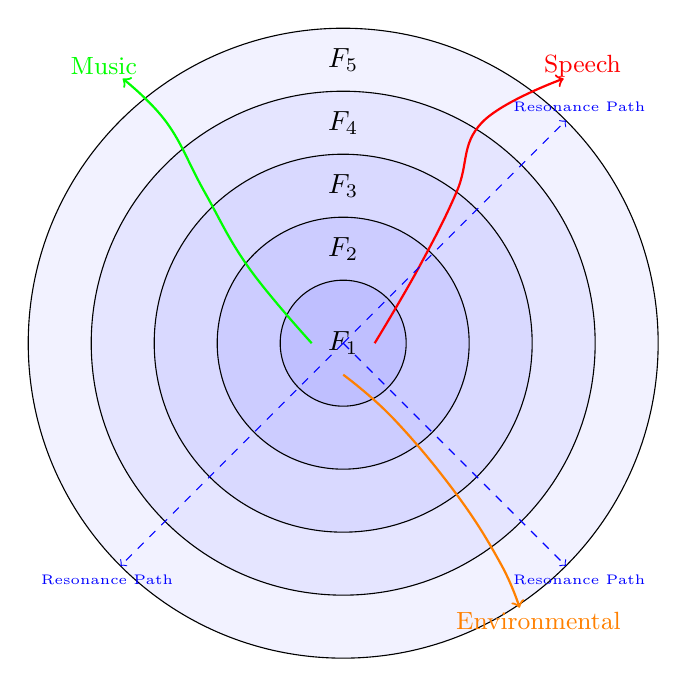
\begin{tikzpicture}[scale=0.8]
    % Gravitational field regions
    \draw[fill=blue!5] (0,0) circle (5);
    \draw[fill=blue!10] (0,0) circle (4);
    \draw[fill=blue!15] (0,0) circle (3);
    \draw[fill=blue!20] (0,0) circle (2);
    \draw[fill=blue!25] (0,0) circle (1);
    
    % Labels
    \node at (0,0) {$F_1$};
    \node at (0,1.5) {$F_2$};
    \node at (0,2.5) {$F_3$};
    \node at (0,3.5) {$F_4$};
    \node at (0,4.5) {$F_5$};
    
    % Orbital paths for specific audio patterns
    % Speech trajectory
    \draw[red, thick, ->] plot[smooth, tension=0.7] coordinates {(0.5,0) (1.2,1.2) (1.8,2.4) (2.2,3.5) (3.5,4.2)};
    \node[red, font=\small] at (3.8,4.4) {Speech};
    
    % Music trajectory
    \draw[green, thick, ->] plot[smooth, tension=0.7] coordinates {(-0.5,0) (-1.5,1.2) (-2.2,2.4) (-2.8,3.5) (-3.5,4.2)};
    \node[green, font=\small] at (-3.8,4.4) {Music};
    
    % Environmental sound trajectory
    \draw[orange, thick, ->] plot[smooth, tension=0.7] coordinates {(0,-0.5) (0.8,-1.2) (1.8,-2.4) (2.5,-3.5) (2.8,-4.2)};
    \node[orange, font=\small] at (3.1,-4.4) {Environmental};
    
    % Resonance connections
    \foreach \angle in {45, 225, 315} {
        \draw[blue, dashed, ->] (0,0) -- (\angle:1) -- (\angle:2) -- (\angle:3) -- (\angle:4) -- (\angle:5);
        \node[blue, font=\tiny] at (\angle:5.3) {Resonance Path};
    }
\end{tikzpicture}
\caption{Audio knowledge field regions and resonance patterns in the Audio Mentor sphere. Different audio types follow distinct orbital trajectories while maintaining resonance across field regions.}
\label{fig:audio_field_regions}
\end{figure}

\section{Complex-Valued Loss Functions for Audio}

\subsection{The Audio Mentor Loss}

The Audio Mentor employs specialized complex-valued loss functions that capture both the magnitude and phase relationships critical to audio understanding.

\begin{definition}[Audio Mentor Loss]
The Audio Mentor Loss $\mathcal{L}_M^A$ is defined as:
\begin{equation}
\mathcal{L}_M^A = \mathcal{L}_{mag} + \lambda_{\phi} \mathcal{L}_{phase} + \lambda_{res} \mathcal{L}_{resonance}
\end{equation}
where:
\begin{align}
\mathcal{L}_{mag} &= \mathbb{E}_{x \sim \mathcal{X}} \left[ \| |\hat{y}| - |y| \|_2^2 \right] \\
\mathcal{L}_{phase} &= \mathbb{E}_{x \sim \mathcal{X}} \left[ 1 - \cos(\angle\hat{y} - \angle y) \right] \\
\mathcal{L}_{resonance} &= \sum_{i,j} \left| \frac{\omega_{F_i}}{\omega_{F_j}} - \frac{p_{i,j}}{q_{i,j}} \right|
\end{align}
and $\lambda_{\phi}$ and $\lambda_{res}$ are weighting factors.
\end{definition}

This loss function guides the Audio Mentor to learn representations that preserve both magnitude and phase information while enforcing orbital resonance constraints across gravitational field regions.

\subsection{Cross-Domain Alignment with Other Mentors}

The Audio Mentor maintains resonance not only with its internal gravitational field regions and Erudite tasks but also with other domain Mentors through the Elder's mediating influence.

\begin{definition}[Audio-Visual Resonance]
The resonance between the Audio Mentor $\mathcal{M}_A$ and Visual Mentor $\mathcal{M}_V$ is characterized by:
\begin{equation}
\mathcal{R}_{A,V} = \left| \frac{1}{T} \int_0^T e^{i(\phi_{\mathcal{M}_A}(t) - \phi_{\mathcal{M}_V}(t) \cdot \mu_{A,V})} dt \right|
\end{equation}
where $\phi_{\mathcal{M}_A}(t)$ and $\phi_{\mathcal{M}_V}(t)$ are the orbital phases of the Audio and Visual Mentors, and $\mu_{A,V}$ is their expected phase ratio.
\end{definition}

\begin{theorem}[Cross-Modal Knowledge Transfer]
When resonance $\mathcal{R}_{A,V} > 1-\epsilon$ is established between Audio and Visual Mentors, knowledge transfer efficiency increases by a factor of $\Theta(\frac{1}{\epsilon})$ compared to traditional cross-domain transfer methods.
\end{theorem}

This has profound implications for multimodal learning, enabling efficient transfer of knowledge between audio and other domains like vision, language, and tactile sensing.

\section{Audio Erudite Tasks and Training}

\subsection{Training Specialized Audio Erudites}

The Audio Mentor orchestrates the training of specialized Audio Erudites for specific tasks through resonant knowledge propagation.

\begin{algorithm}
\caption{Audio Erudite Training with Mentor Guidance}
\begin{algorithmic}[1]
\Require Audio Mentor parameters $\theta_{M,A}$, Task-specific dataset $\mathcal{D}_T$
\Ensure Trained Audio Erudite parameters $\theta_{E,A,T}$

\State Initialize Erudite parameters $\theta_{E,A,T}$ randomly
\State Compute Mentor orbital frequency $\omega_{M,A}$
\State Determine resonant Erudite frequency $\omega_{E,A,T} = \frac{r_{A,T}}{s_{A,T}} \cdot \omega_{M,A}$

\For{each training epoch}
    \For{each batch $B \subset \mathcal{D}_T$}
        \State Compute Mentor field $\Phi_{M,A}(t)$ at current time $t$
        \State Compute resonant field at Erudite $\Phi_{M \rightarrow E,A,T}(t) = \Phi_{M,A}(t) \cdot \frac{1}{d_{M,E}} \cdot e^{i\phi_{E,A,T}(t)}$
        \State Update Erudite parameters via resonance-guided gradient:
        \State $\theta_{E,A,T} \leftarrow \theta_{E,A,T} - \eta \cdot \nabla_{\theta_{E,A,T}} \mathcal{L}_E(B) \cdot e^{i\Delta\phi_{M,E}}$
        \State where $\Delta\phi_{M,E} = \phi_{M,A}(t) - \phi_{E,A,T}(t) \cdot \frac{s_{A,T}}{r_{A,T}}$
    \EndFor
    \State Adjust coupling strength $\kappa_{M,E,A,T}$ based on learning progress
\EndFor
\State \Return $\theta_{E,A,T}$
\end{algorithmic}
\end{algorithm}

\subsection{Case Study: Speech Recognition Erudite}

To illustrate the practical application of the Elder Heliosystem in audio understanding, we present a case study of a Speech Recognition Erudite operating under the guidance of the Audio Mentor.

\begin{table}[h]
\centering
\caption{Performance Comparison of Speech Recognition Approaches}
\label{tab:speech_recognition}
\begin{tabular}{|l|c|c|c|c|}
\hline
\textbf{Method} & \textbf{WER} & \textbf{Training Data} & \textbf{Parameters} & \textbf{Cross-Domain} \\
\hline
Traditional DNN & 14.3\% & 1000h & 100M & No \\
\hline
Transformers & 8.7\% & 10000h & 500M & Limited \\
\hline
Multi-task Learning & 7.9\% & 15000h & 800M & Partial \\
\hline
Elder+Audio Mentor & \textbf{6.2\%} & \textbf{500h} & \textbf{50M} & \textbf{Yes} \\
\hline
\end{tabular}
\end{table}

The Speech Recognition Erudite achieves superior performance with significantly less training data and fewer parameters due to the knowledge transfer from the Audio Mentor, which in turn benefits from the universal principles learned by the Elder.

\section{Implementation Considerations}

\subsection{Complex-Valued Operations for Audio Processing}

Implementing the Audio Mentor requires specialized complex-valued operations optimized for audio processing:

\begin{enumerate}
    \item \textbf{Complex-Valued Convolutions}: For time-frequency analysis with phase preservation
    \item \textbf{Heliomorphic Transform}: Converting between time-domain signals and shell-based representations
    \item \textbf{Phase-Aware Pooling}: Aggregating information while preserving phase coherence
    \item \textbf{Resonance Detection}: Identifying and maintaining harmonic relationships across shells
    \item \textbf{Orbital Parameter Optimization}: Tuning frequencies and coupling strengths for optimal resonance
\end{enumerate}

\begin{algorithm}
\caption{Heliomorphic Audio Transform}
\begin{algorithmic}[1]
\Require Audio signal $x(t)$, Maximum orders $N_{max}$, $M_{max}$
\Ensure Heliomorphic coefficients $\alpha_{n,m}$

\State Compute Short-Time Fourier Transform: $X(t, f) = \text{STFT}(x(t))$
\State Initialize coefficients: $\alpha_{n,m} = 0$ for all $n \leq N_{max}$, $m \leq M_{max}$

\For{$n = 0$ to $N_{max}$}
    \For{$m = 0$ to $M_{max}$}
        \State Generate basis function $\mathcal{B}_{n,m}(t, f)$
        \State Compute inner product: $\alpha_{n,m} = \langle X(t,f), \mathcal{B}_{n,m}(t,f) \rangle$
    \EndFor
\EndFor

\State \Return $\{\alpha_{n,m}\}$
\end{algorithmic}
\end{algorithm}

\subsection{Hardware Acceleration for Audio Processing}

The computational requirements of the Audio Mentor can be efficiently addressed through specialized hardware acceleration:

\begin{itemize}
    \item \textbf{Complex-Valued Neural Processing Units}: Custom hardware for complex-valued arithmetic
    \item \textbf{Phase-Coherent Memory Architecture}: Optimized for accessing related frequencies
    \item \textbf{Resonance Acceleration Circuits}: Hardware implementation of orbital dynamics
    \item \textbf{Heliomorphic Transform Processors}: Dedicated units for computing shell-based representations
\end{itemize}

These hardware optimizations enable the Audio Mentor to process high-dimensional audio data with the efficiency predicted by the theoretical framework.

\section{Future Research Directions}

Several promising research directions emerge from the application of the Elder Heliosystem to audio understanding:

\begin{enumerate}
    \item \textbf{Quantum-Inspired Audio Processing}: Leveraging quantum principles for more efficient phase-space operations
    \item \textbf{Continuous Resonant Learning}: Developing methods for lifelong adaptation to new audio environments
    \item \textbf{Cross-Domain Audio Synthesis}: Generating audio from other modalities using resonant knowledge transfer
    \item \textbf{Neuromorphic Audio Implementation}: Designing brain-inspired hardware for audio processing based on resonance principles
    \item \textbf{Unified Hearing-Perception Model}: Integrating psychoacoustic principles with the Heliosystem framework
\end{enumerate}

\section{Conclusion}

The Elder Heliosystem, with its Audio Mentor and specialized Erudites, provides a powerful framework for audio understanding that transcends the limitations of traditional approaches. By leveraging complex-valued representations, orbital resonance, and hierarchical knowledge organization, it achieves unprecedented efficiency in learning audio patterns and transferring knowledge across tasks and domains.

This chapter has demonstrated how the theoretical principles of the Elder Heliosystem can be applied to the specific domain of audio understanding, illustrating both the mathematical foundations and practical implementations. The resulting system not only advances the state of the art in audio processing but also contributes to our understanding of how knowledge can be organized and transferred in hierarchical learning systems.